\begin{comment}
Multicore architectures 
cache system
sharing and false sharing
existing tools for false sharing
limitations
contributions
structures
\end{comment}

%% TONGPING: to be honest, I think that we are talking too much on the foreword of introduction. Can we make it shorter?
Modern computer systems, such as server nodes, desktops, and smart phones, employ multiple cores to achieve high parallelism. 
To bridge the speed gap between CPU and main memory, multi-level cache hierarchies are used to block data for fast accesses. Typically in the memory hierarchy, there are private layers associated with each core and shared layers between cores. For example, Intel Sandy Bridge processors have private L1 and L2 caches, as well as shared L3 caches. Moreover, IBM POWER8 processors have L1, L2 private caches, and L3, L4 shared caches.
To facilitate programming and guarantee the correctness, there are complex cache coherency protocols~\cite{MESI} implemented in the hierarchy.

The complex memory hierarchies in multi-core systems may suffer from various performance issues, such as poor data locality~\cite{ibs-sc,ibs-ispass}, intensive cache contention~\cite{ibs-sc2}, and bandwidth underutilization~\cite{Dramon}. Among them, false sharing is a common programming flaw that can significant hurt a parallel program's performance and scalability. % What is the relationship? 
False sharing occurs between threads, when these threads (1) run on cores with private caches, (2) access different words of a cache line, unlike true sharing between threads, which access the same word, and (3) at least one access is a write. Given the cache coherence protocol, threads with writing the words keep invalidating the cache line in all private caches and flushing the data to the shared caches. Thus, when some threads use the data, they need to load the data from the shared cache, rather than the fast private one.

%Multicore processors are ubiquitous, from phones, desktops, to high-end servers.
%False sharing occurs when multiple tasks, running on different cores with private L1 caches, access logically independent words in the same cache line. When a thread modifies data of a cache line, the underlying cache coherence protocol (inside hardware) silently invalidates the duplicates of this cache line on other cores. Unnecessary synchronizations caused by false sharing can dramatically degrade the performance of parallel software by up to an order of magnitude ~\cite{falseshare:effect}. A simple example shown in Figure~\ref{fig:penalty} also exemplifies this catastrophic performance effect of false sharing. Figure~\ref{} shows how false sharing occurs in a typical multi-core platform.


%The hardware trend, including adding more cores into the same machine, introducing the Non-Uniform-Memory-Access (NUMA) architecture, or increasing the size of a cache line, will further degrade the performance of false sharing problems, making the task of detecting even more urgent. 

\begin{figure*}[htbp]
\centering
\subfigure[Parallel Programs]{%
   \label{fig:penaltycode}
   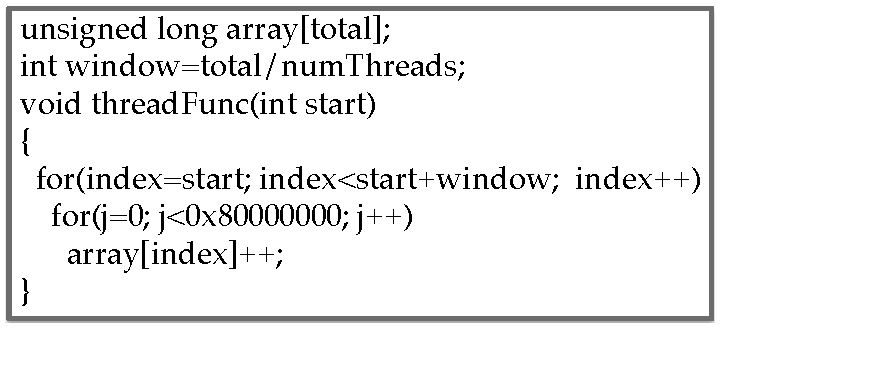
\includegraphics[width=2.8in]{figure/fscode}

}%
\hspace{30pt}
\subfigure[Performance Degradation]{%
   \label{fig:penaltyfig}
   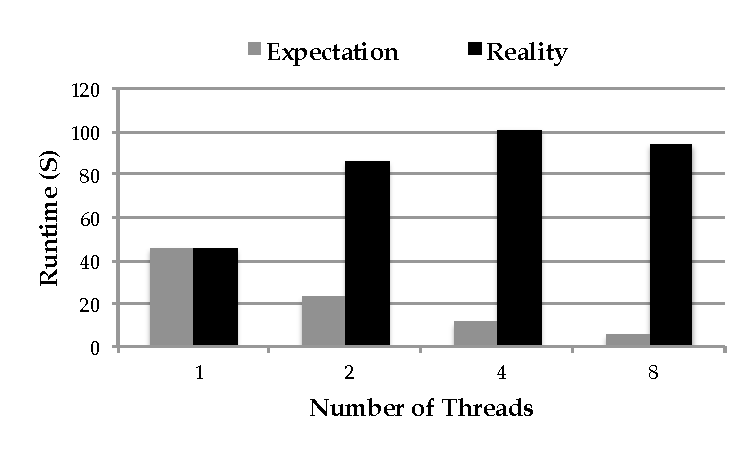
\includegraphics[width=2.4in]{figure/penalty}
}
\caption{
A false sharing example inside a multithreaded program (a) causes $13\times$ performance degradation (b) on a 8-core machine.
\label{fig:penalty}}
\end{figure*}

% Now we will talk about existing tools. 
As a concrete example, as shown in Figure~\ref{fig:penalty}, careless code design can lead to false sharing: multiple threads may simultaneously access adjacent elements of {\tt array} that reside in the same cache line. As a result shown in Figure~\ref{fig:penaltyfig},  the performance of this program (in red) is much worse than the expected (in green). When running with eight threads, this program actually runs around $13\times$ slower than its expectation (without false sharing).  Therefore, it is very important to eliminate false sharing to obtain high performance and scalability. 
Unlike true sharing, false sharing is generally avoidable. Since threads unnecessarily share the same cache line, we can pad the data so that  each thread can be forced to access a different cache line. Although the solution of fixing false sharing is straightforward, detecting them is difficult and even impossible with manual effort only, especially for a program with  thousands or millions lines of code. Thus, it is very important to employ tools to pinpoint false sharing and provide insightful optimization guidance.

However, existing generic performance tools do not provide details about false sharing. For example, well-known profilers such as gprof~\cite{gprof}, HPCToolkit~\cite{ibs-sc}, TAU~\cite{Malony-etal:2008:TAU}, and VTune~\cite{Intel:VTune} report time consumption and cache miss counts, but do not point that whether the long running time and large amount of cache misses are caused by false sharing or not. On the other hand, existing false sharing detection tools fall short in several ways. First, some tools~\cite{falseshare:binaryinstrumentation1,detect:ptu,detect:intel,falseshare:binaryinstrumentation2,DProf, qinzhao, OSdetection, mldetect, Wicaksono11detectingfalse, openmp} do not distinguish true and false sharing, while requiring unnecessary manual efforts to identify optimization opportunities. Second, some tools~\cite{falseshare:binaryinstrumentation1,falseshare:binaryinstrumentation2,falseshare:simulator, Predator} introduce high runtime overhead, preventing them from uses in deployment environemnt. Third, some tools require special features from OS~\cite{OSdetection}, compilers~\cite{Predator}, and applications~\cite{Sheriff}. Fourth, to the best of our knowledge, no prior tool assesses the benefit from eliminating the false sharing. Without this information, many optimization efforts may lead to trivial performance improvement.

\vspace{0.2in}

To address these issues, we develop \cheetah{} with the following three contributions:
\begin{itemize} 

% The first one is overrated. We can't do that. 
\item \cheetah{} can report precise information about false sharing problems. Like those precise tools, e.g. Sheriff~\cite{Sheriff} and Predator~\cite{Predator}, it will pinpoint the lines of code where those variables or objects have false sharing problems. More than that, \cheetah{} can further pinpoint statements exercising false sharing problems, which can help programmers fix found problems. 

\sloppy
\item Based on hardware performance monitoring units (PMU), \cheetah{} significantly reduces the runtime overhead of detection, with only 5\% average performance overhead and 10\% maximum overhead. The performance overhead is similar to recent work~\cite{mldetect, openmp}, but with more precise information and more effectiveness.
  
\item Unlike all existing tools, \Cheetah{} can quantify the performance impact of false sharing instances based on the memory access latency information provided by PMU. By ruling out trivial cases, \Cheetah{} can avoid unnecessary manual effort as much as possible. 
\end{itemize}
\cheetah{} is a compiler-, OS-, and application-independent tool that works on fully optimized binaries and out-of-box Linux with the driver to hardware PMU~\footnote{The access to PMU is in the mainline of Linux kernel since 2.6.32.}. To evaluate \cheetah{}, we apply it to a number of well-known benchmarks from Phoenix and PARSEC suites. Experiments show that \cheetah{} can efficiently and effectively guide us fix false sharing problems with significant performance improvement.

The remainder of this paper is organized as follows. Section~\ref{sec:overview} introduces the background of false sharing and \cheetah{}'s basic idea. Section~\ref{sec:implement} describes implementations in detail. Section~\ref{sec:eval} presents experimental results, including effectiveness, performance overhead, and memory overhead. Section~\ref{sec:relatedwork} discusses some related work and Section~\ref{sec:relatedwork} concludes this paper. 



